%==============================================================
%  EE201 -- Circuit Theory I
%  Lecture 13 : Input Resistance and the Delta-Y Transform
%  M. Mert Ankaralı, METU EEE
%
%  Compile:  ./build.sh      (or: pdflatex EE201_Lecture_13.tex, twice)
%==============================================================
\documentclass[11pt,a4paper]{article}

%-------------------- packages --------------------------------
\usepackage[T1]{fontenc}
\usepackage[utf8]{inputenc}
\usepackage[english]{babel}
\usepackage{lmodern}
\usepackage[margin=2.3cm,top=2.0cm,bottom=1.9cm,headheight=14pt,headsep=9pt]{geometry}
\usepackage{amsmath,amssymb}
\usepackage{array,booktabs,tabularx}
\usepackage{enumitem}
\usepackage{needspace}
\usepackage[table]{xcolor}
\usepackage{fancyhdr}
\usepackage{titlesec}
\usepackage{graphicx}
\usepackage[most]{tcolorbox}
\usepackage{tikz}
\usepackage[american,siunitx]{circuitikz}
\usetikzlibrary{matrix,arrows.meta,positioning,calc,decorations.pathmorphing,decorations.pathreplacing,decorations.markings,patterns,shapes.geometric}
\usepackage[colorlinks=true,allcolors=metured,breaklinks=true]{hyperref}

%-------------------- colour system ---------------------------
% One colour per physical quantity, used identically in the slides.
\definecolor{metured}{RGB}{155,27,48}    % headings, structure
\definecolor{metugray}{RGB}{88,89,91}
\definecolor{ccur}{RGB}{0,102,170}       % CURRENT  -- blue
\definecolor{cvolt}{RGB}{214,120,0}      % VOLTAGE  -- orange
\definecolor{cpow}{RGB}{23,128,74}       % POWER / ENERGY -- green
\definecolor{ccharge}{RGB}{124,60,160}   % CHARGE   -- purple
\definecolor{cflux}{RGB}{0,138,138}      % FLUX -- teal
\definecolor{boxgray}{RGB}{245,245,245}
\definecolor{copper}{RGB}{184,98,30}

\newcommand{\Icol}[1]{\textcolor{ccur}{#1}}
\newcommand{\Vcol}[1]{\textcolor{cvolt}{#1}}
\newcommand{\Pcol}[1]{\textcolor{cpow}{#1}}
\newcommand{\Qcol}[1]{\textcolor{ccharge}{#1}}
\newcommand{\Fcol}[1]{\textcolor{cflux}{#1}}

%-------------------- units (no siunitx dependency) -----------
\newcommand{\uni}[1]{\,\mathrm{#1}}
\newcommand{\A}{\uni{A}}   \newcommand{\V}{\uni{V}}
\newcommand{\W}{\uni{W}}   \newcommand{\J}{\uni{J}}
\newcommand{\Cb}{\uni{C}}  \newcommand{\s}{\uni{s}}
\newcommand{\Sie}{\uni{S}} \newcommand{\Wb}{\uni{Wb}}

%-------------------- layout ----------------------------------
\pagestyle{fancy}
\fancyhf{}
\lhead{\small\textcolor{metugray}{EE201 -- Circuit Theory I}}
\rhead{\small\textcolor{metugray}{Lecture 13: Input Resistance and the $\Delta$--Y Transform}}
\cfoot{\small\thepage}
\renewcommand{\headrulewidth}{0.4pt}

\titleformat{\section}{\large\bfseries\color{metured}}{\thesection.}{0.6em}{}
\titleformat{\subsection}{\normalsize\bfseries\color{metugray}}{\thesubsection.}{0.6em}{}
\titlespacing*{\section}{0pt}{1.4ex plus .3ex}{0.7ex}
\titlespacing*{\subsection}{0pt}{1.1ex plus .2ex}{0.5ex}

\setlist[itemize]{itemsep=2pt,topsep=3pt,parsep=0pt,leftmargin=1.5em}
\setlist[enumerate]{itemsep=2pt,topsep=3pt,parsep=0pt,leftmargin=1.7em}
\setlength{\parindent}{0pt}
\setlength{\parskip}{0.7ex plus .1ex}
\raggedbottom
\widowpenalty=10000
\clubpenalty=10000
\brokenpenalty=10000

%-------------------- boxes -----------------------------------
\newtcolorbox{definitionbox}[1]{enhanced,
  colback=metured!4, colframe=metured, boxrule=0.9pt,
  fonttitle=\bfseries, title={#1}, arc=2pt,
  left=7pt,right=7pt,top=5pt,bottom=5pt, before skip=7pt, after skip=7pt,
  before upper={\setlength{\parskip}{0.6ex plus .1ex}}}

\newtcolorbox{ideabox}[1][Key idea]{enhanced,
  colback=ccur!5, colframe=ccur, boxrule=0.9pt,
  fonttitle=\bfseries, title={#1}, arc=2pt,
  left=7pt,right=7pt,top=5pt,bottom=5pt, before skip=7pt, after skip=7pt,
  before upper={\setlength{\parskip}{0.6ex plus .1ex}}}

\newtcolorbox{examplebox}[1][Example]{enhanced,
  colback=cpow!4, colframe=cpow, boxrule=0.9pt,
  fonttitle=\bfseries, title={#1}, arc=2pt,
  left=7pt,right=7pt,top=5pt,bottom=5pt, before skip=7pt, after skip=7pt,
  before upper={\setlength{\parskip}{0.6ex plus .1ex}}}

\newtcolorbox{cautionbox}[1][Careful]{enhanced,
  colback=cvolt!6, colframe=cvolt, boxrule=0.9pt,
  fonttitle=\bfseries, title={#1}, arc=2pt,
  left=7pt,right=7pt,top=5pt,bottom=5pt, before skip=7pt, after skip=7pt,
  before upper={\setlength{\parskip}{0.6ex plus .1ex}}}

%-------------------- circuitikz defaults ---------------------
%  voltage sources: smaller + and - inside the circle, further apart
\ctikzset{bipoles/vsourceam/inner plus={\tiny$+$},
          bipoles/vsourceam/inner minus={\tiny$\vphantom{+}-$},
          bipoles/vsourceam/margin=0.85,
          bipoles/cvsourceam/inner plus={\tiny$+$},
          bipoles/cvsourceam/inner minus={\tiny$\vphantom{+}-$},
          bipoles/cvsourceam/margin=0.85}
\ctikzset{bipoles/length=0.9cm, color=black,
          label/align=straight,
          bipoles/generic/height=0.28, bipoles/generic/width=0.62}
\tikzset{
  iar/.style={-{Stealth[length=2.2mm]}, ccur, thick},
  pol/.style={font=\small, text=cvolt},
  glab/.style={font=\footnotesize, text=metured},
  ttl/.style={font=\scriptsize\bfseries, text=metugray},
  capn/.style={font=\scriptsize, text=metugray, align=center},
  bigarr/.style={-{Stealth[length=3mm]}, very thick, metugray},
  gnode/.style={circle, fill=metured, inner sep=0pt, minimum size=4.4pt},
  nlab/.style={circle, draw=metured, text=metured, font=\scriptsize, inner sep=0.7pt},
  blab/.style={font=\footnotesize, text=black!80},
  gbr/.style={black!75, thick, postaction={decorate, decoration={markings,
      mark=at position 0.56 with {\arrow{Stealth[length=2.5mm]}}}}},
  apbr/.style={ccur, line width=1.7pt, postaction={decorate, decoration={markings,
      mark=at position 0.56 with {\arrow{Stealth[length=2.8mm]}}}}},
  hal/.style={draw=cpow!60, line width=6pt, opacity=0.35, line cap=round, line join=round},
  elem/.style={draw=metugray, thick, fill=metulight},
}
\definecolor{metulight}{RGB}{243,240,241}

%-------------------- Lecture 13 circuit macros ---------------
\newcommand{\ohm}{\,\Omega}
\newcommand{\yes}{\textcolor{cpow}{\checkmark}}
\newcommand{\e}[1]{\textcolor{cvolt}{e_{#1}}}
\newcommand{\nd}[1]{\tikz[baseline=(c.base)]\node[nlab](c){#1};}
\newcommand{\nodev}[3]{\fill (#1) circle (1.7pt) node[#2, inner sep=2pt, font=\small, text=cvolt] {#3};}
\newcommand{\gnd}[2]{\draw (#1,#2) -- ++(0,-0.2) node[ground] {};}
\newcommand{\Rin}{R_{\mathrm{in}}}
%  Sum of the Delta resistors
\newcommand{\SD}{R_A + R_B + R_C}
\tikzset{tlab/.style={font=\small\bfseries, text=black!80},
         hterm/.style={circle, draw=metured, line width=1.6pt, minimum size=9pt, inner sep=0pt},
         sdel/.style={draw=metured, line width=5pt, opacity=0.25, line join=round, line cap=round},
         swye/.style={draw=ccur, line width=5pt, opacity=0.25, line join=round, line cap=round}}

%  A one-port N (box, text #1) with terminals a, b on the right; port current i into a, voltage v
\newcommand{\oneport}[2][1.9]{%
  \draw[elem] (0,0) rectangle (#1,2);
  \node[align=center, font=\small] at ({#1/2},1) {#2};
  \begin{scope}[shift={(#1-1.9,0)}]
  \draw (1.9,1.7) -- (3.0,1.7) node[ocirc] {} node[right, tlab] {a};
  \draw (1.9,0.3) -- (3.0,0.3) node[ocirc] {} node[right, tlab] {b};
  \draw[iar] (2.75,1.95) -- (2.2,1.95); \node[font=\small, text=ccur] at (2.48,2.2) {$i$};
  \node[pol] at (2.6,1.4) {$+$}; \node[pol] at (2.6,0.6) {$-$};
  \node[font=\small, text=cvolt] at (2.6,1.0) {$v$};
  \end{scope}}
%  A single resistor R_in between terminals a, b
\newcommand{\rinres}{%
  \draw (1.1,1.7) -- (0,1.7) to[R, l_=$\Rin$] (0,0.3) -- (1.1,0.3);
  \draw (1.1,1.7) node[ocirc] {} node[right, tlab] {a};
  \draw (1.1,0.3) node[ocirc] {} node[right, tlab] {b};}

%  Test source configurations.  #1 = 0: N with 1 A (I);  1: R_in with 1 A (II)
\newcommand{\testcfg}[1]{%
  \ifnum#1=0
    \draw[elem] (0,0) rectangle (1.5,2); \node at (0.75,1) {$N$};
    \draw (1.5,1.7) -- (2.9,1.7); \draw (1.5,0.3) -- (2.9,0.3);
    \draw (2.9,0.3) to[american current source, l_=$1\A$] (2.9,1.7);
    \node[pol] at (2.05,1.35) {$+$}; \node[pol] at (2.05,0.65) {$-$};
    \node[font=\small, text=cvolt] at (2.05,1.0) {$v_{\mathrm{I}}$};
    \fill (2.9,1.7) circle (1.6pt); \fill (2.9,0.3) circle (1.6pt);
  \else
    \draw (2.9,1.7) -- (0.5,1.7) to[R, l_=$\Rin$] (0.5,0.3) -- (2.9,0.3);
    \draw (2.9,0.3) to[american current source, l_=$1\A$] (2.9,1.7);
    \node[pol] at (1.75,1.35) {$+$}; \node[pol] at (1.75,0.65) {$-$};
    \node[font=\small, text=cvolt] at (1.75,1.0) {$v_{\mathrm{II}}$};
    \fill (2.9,1.7) circle (1.6pt); \fill (2.9,0.3) circle (1.6pt);
  \fi}

%  Example 13.1: a CCVS (3/2) i_x, 3 Ohm, 2 Ohm; port a-b on the right.
%  #1 = 0: bare, R_in = ?;  1: with the 1 A test source, the ground and e_1
\newcommand{\exR}[1]{%
  \draw (0,2) to[american controlled voltage source, l_=$\Vcol{\tfrac32\,i_x}$] (0,0);
  \draw (0,2) to[R, l=$3\ohm$] (2.4,2) to[R, l_=$2\ohm$] (2.4,0);
  \draw (2.4,2) -- (4.6,2); \draw (0,0) -- (4.6,0);
  \draw[iar] (4.3,0.28) -- (3.55,0.28); \node[font=\small, text=ccur] at (3.92,0.55) {$i_x$};
  \fill (2.4,2) circle (1.7pt); \fill (2.4,0) circle (1.7pt);
  \ifnum#1=0
    \draw (4.6,2) node[ocirc] {} node[above, tlab] {a};
    \draw (4.6,0) node[ocirc] {} node[below, tlab] {b};
    \draw[bigarr] (5.8,1) -- (4.9,1); \node[right] at (5.8,1) {$\Rin = \ ?$};
  \else
    \draw (4.6,0) to[american current source, l_=$1\A$] (4.6,2);
    \fill (4.6,2) circle (1.7pt); \fill (4.6,0) circle (1.7pt);
    \node[font=\small, text=cvolt, above] at (2.4,2.05) {$e_1$};
    \node[pol] at (3.75,1.65) {$+$}; \node[pol] at (3.75,0.95) {$-$};
    \node[font=\small, text=cvolt] at (3.75,1.3) {$v_{\mathrm{I}}$};
    \gnd{2.4}{0}
  \fi}

%  Three-terminal circuits.  Terminals A (0,0), B (3,0), C (1.5,2.5).
%  #1 = 0: no highlight;  1: A and B;  2: B and C;  3: C and A
\newcommand{\hlpair}[1]{%
  \ifcase#1\or
    \node[hterm] at (0,0) {}; \node[hterm] at (3,0) {};
  \or
    \node[hterm] at (3,0) {}; \node[hterm] at (1.5,2.5) {};
  \or
    \node[hterm] at (1.5,2.5) {}; \node[hterm] at (0,0) {};
  \fi}
%  Delta: R_C between A and B, R_A between B and C, R_B between C and A
\newcommand{\Dlt}[1]{%
  \draw (0,0) to[R] (3,0) to[R] (1.5,2.5) to[R] (0,0);
  \node[font=\small] at (1.5,-0.45) {$R_C$};
  \node[font=\small] at (2.85,1.6) {$R_A$};
  \node[font=\small] at (0.15,1.6) {$R_B$};
  \draw (0,0) node[ocirc] {} node[left=2pt, tlab] {A};
  \draw (3,0) node[ocirc] {} node[right=2pt, tlab] {B};
  \draw (1.5,2.5) node[ocirc] {} node[above=2pt, tlab] {C};
  \hlpair{#1}}
%  Y: R_1 at A, R_2 at B, R_3 at C, centre (1.5,0.95)
\newcommand{\Wye}[1]{%
  \draw (0,0) to[R] (1.5,0.95); \draw (3,0) to[R] (1.5,0.95);
  \draw (1.5,2.5) to[R] (1.5,0.95);
  \fill (1.5,0.95) circle (1.6pt);
  \node[font=\small] at (0.55,0.98) {$R_1$};
  \node[font=\small] at (2.45,0.98) {$R_2$};
  \node[font=\small] at (1.95,1.8) {$R_3$};
  \draw (0,0) node[ocirc] {} node[left=2pt, tlab] {A};
  \draw (3,0) node[ocirc] {} node[right=2pt, tlab] {B};
  \draw (1.5,2.5) node[ocirc] {} node[above=2pt, tlab] {C};
  \hlpair{#1}}
%  Equal resistors: #1 = 0: Delta with R, R, R;  1: Y with labels #2
\newcommand{\Dltq}{%
  \draw (0,0) to[R] (3,0) to[R] (1.5,2.5) to[R] (0,0);
  \node[font=\small] at (1.5,-0.45) {$R$};
  \node[font=\small] at (2.8,1.6) {$R$};
  \node[font=\small] at (0.2,1.6) {$R$};
  \foreach \p in {(0,0),(3,0),(1.5,2.5)} \draw \p node[ocirc] {};}
\newcommand{\Wyeq}[1]{%
  \draw (0,0) to[R] (1.5,0.95); \draw (3,0) to[R] (1.5,0.95);
  \draw (1.5,2.5) to[R] (1.5,0.95);
  \fill (1.5,0.95) circle (1.6pt);
  \node[font=\small] at (0.5,1.0) {$#1$};
  \node[font=\small] at (2.5,1.0) {$#1$};
  \node[font=\small] at (2.0,1.8) {$#1$};
  \foreach \p in {(0,0),(3,0),(1.5,2.5)} \draw \p node[ocirc] {};}

%  Example 13.2: a bridge between the terminals (top and bottom on the left).
%  #1 = 0: bare;  1: node names and the Delta A-B-C highlighted;  2: after Delta -> Y
\newcommand{\exBr}[1]{%
  \ifnum#1<2
    \draw (-1.3,4.0) -- (2,4.0) -- (2,3.4); \draw (-1.3,0) -- (2,0);
    \draw (-1.3,4.0) node[ocirc] {}; \draw (-1.3,0) node[ocirc] {};
    \draw (2,3.4) to[R] (0,1.7) to[R] (2,0);
    \draw (2,3.4) to[R] (4,1.7) to[R] (2,0);
    \draw (0,1.7) to[R] (4,1.7);
    \foreach \p in {(2,3.4),(0,1.7),(4,1.7),(2,0)} \fill \p circle (1.7pt);
    \node[font=\small] at (0.4,3.05) {$7\ohm$};
    \node[font=\small] at (3.6,3.05) {$20\ohm$};
    \node[font=\small] at (2,2.15) {$10\ohm$};
    \node[font=\small] at (0.4,0.3) {$50\ohm$};
    \node[font=\small] at (3.6,0.3) {$40\ohm$};
    \ifnum#1=1
      \draw[sdel] (0,1.7) -- (4,1.7) -- (2,0) -- cycle;
      \node[tlab, left] at (-0.1,1.7) {A}; \node[tlab, right] at (4.1,1.7) {B};
      \node[tlab, below right] at (2.05,-0.05) {C};
    \fi
  \else
    \draw (-1.3,4.0) -- (2,4.0) -- (2,3.4); \draw (-1.3,-0.6) -- (2,-0.6);
    \draw (-1.3,4.0) node[ocirc] {}; \draw (-1.3,-0.6) node[ocirc] {};
    \draw (2,3.4) to[R] (0,2.0) to[R] (2,0.9);
    \draw (2,3.4) to[R] (4,2.0) to[R] (2,0.9);
    \draw (2,0.9) to[R] (2,-0.6);
    \draw[swye] (0,2.0) -- (2,0.9) -- (4,2.0); \draw[swye] (2,0.9) -- (2,-0.6);
    \foreach \p in {(2,3.4),(0,2.0),(4,2.0),(2,0.9),(2,-0.6)} \fill \p circle (1.7pt);
    \node[font=\small] at (0.45,3.15) {$7\ohm$};
    \node[font=\small] at (3.6,3.15) {$20\ohm$};
    \node[font=\small, text=ccur] at (0.65,0.9) {$5\ohm$};
    \node[font=\small, text=ccur] at (3.35,0.9) {$4\ohm$};
    \node[font=\small, text=ccur] at (2.7,0.15) {$20\ohm$};
    \node[tlab, left] at (-0.1,2.0) {A}; \node[tlab, right] at (4.1,2.0) {B};
    \node[tlab, below right] at (2.05,-0.65) {C};
  \fi}
\begin{document}

%-------------------- title block -----------------------------
\begin{center}
\begin{tcolorbox}[enhanced, colback=metured!5, colframe=metured, boxrule=1pt,
                  arc=3pt, left=10pt,right=10pt,top=7pt,bottom=7pt, width=\textwidth]
\begin{center}
  {\small\scshape Middle East Technical University}\\[2pt]
  {\small\scshape Department of Electrical and Electronics Engineering}\\[7pt]
  {\Large\bfseries\color{metured} EE201 -- Circuit Theory I}\\[4pt]
  {\large\bfseries Lecture 13: Input Resistance and the $\boldsymbol{\Delta}$--Y Transform}\\[6pt]
  {\small M. Mert Ankaralı}
\end{center}
\end{tcolorbox}
\end{center}
\vspace{-0.5em}

\begin{center}
\small
\begin{tabular}{@{}l l@{}}
\toprule
\multicolumn{2}{@{}l}{\textbf{Colour code used in these notes and in the slides}}\\
\midrule
\Icol{$\blacksquare$}~current $i$ \quad
\Vcol{$\blacksquare$}~voltage $v$, node voltage $e$ &
\textcolor{metured}{$\blacksquare$}~a $\Delta$ \quad \Icol{$\blacksquare$}~a Y\\
\bottomrule
\end{tabular}
\end{center}

\textbf{Motivation.} Previously, we simplified circuits with equivalent one-ports: series and
parallel connections and source transformation. Two cases need more. A one-port with
dependent sources is not a series--parallel connection of resistors. A bridge has no two
resistors in series or in parallel. This lecture finds one equivalent resistor in both cases:
the \textbf{input resistance} of a one-port, and the \textbf{$\boldsymbol{\Delta}$--Y transform}
of three resistors.

%==============================================================
\section{The input resistance of a one-port}

\begin{definitionbox}{Input resistance}
\begin{minipage}[c]{0.5\linewidth}
Let a one-port $N$ contain only LTI resistors, LTI dependent sources and ideal transformers,
with every control variable inside $N$. Then $N$ is equivalent to a single LTI resistor
$\Rin$, the \textbf{input resistance} of $N$: \ $\Vcol{v} = \Rin\,\Icol{i}$ at its port.
\end{minipage}\hfill
\begin{minipage}[c]{0.46\linewidth}
\centering
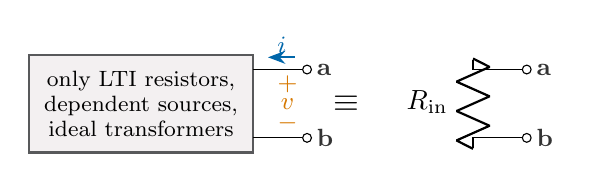
\begin{tikzpicture}[scale=0.62]
  \oneport[4.6]{\footnotesize only LTI resistors,\\[-2pt] \footnotesize dependent sources,\\[-2pt]
    \footnotesize ideal transformers}
  \node[font=\large] at (6.5,1) {$\equiv$};
  \begin{scope}[shift={(9.1,0)}]
    \rinres
  \end{scope}
\end{tikzpicture}
\end{minipage}
\end{definitionbox}

\begin{minipage}[c]{0.5\linewidth}
With dependent sources, series and parallel rules are not enough to find $\Rin$. A
\textbf{test source} finds it. Connect a $1\A$ current source to the port of $N$ (circuit I)
and to $\Rin$ (circuit II). Since $N \equiv \Rin$, the port voltages are equal:
$\Vcol{v_{\mathrm{I}}} = \Vcol{v_{\mathrm{II}}} = \Rin \cdot 1\A$, so
\[
  \Rin = \frac{\Vcol{v_{\mathrm{I}}}}{1\A}: \quad \text{solve circuit (I)}.
\]
\end{minipage}\hfill
\begin{minipage}[c]{0.46\linewidth}
\centering
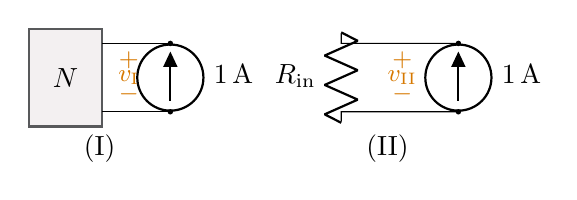
\begin{tikzpicture}[scale=0.62]
  \testcfg{0} \node at (1.45,-0.45) {(I)};
  \begin{scope}[shift={(5.9,0)}]
    \testcfg{1} \node at (1.45,-0.45) {(II)};
  \end{scope}
\end{tikzpicture}
\end{minipage}

\medskip
\begin{examplebox}[Example 13.1 --- an input resistance]
\begin{minipage}[c]{0.46\linewidth}
\centering
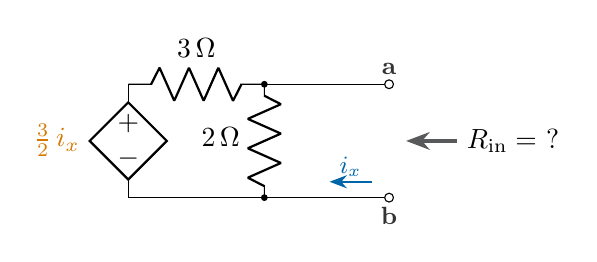
\begin{tikzpicture}[scale=0.72]
  \exR{0}
\end{tikzpicture}\\[6pt]
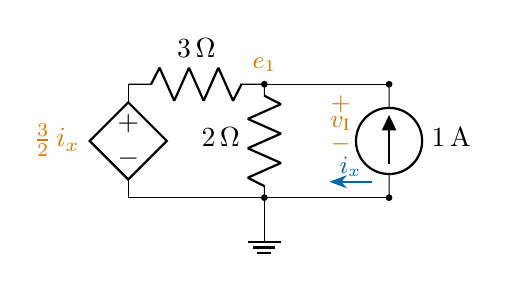
\begin{tikzpicture}[scale=0.72]
  \exR{1}
\end{tikzpicture}
\end{minipage}\hfill
\begin{minipage}[c]{0.5\linewidth}
\textbf{Question.} Find $\Rin$.

\textbf{Answer.} Connect a $1\A$ test source and take the bottom node as the ground. KCL at
node 1:
\[
  \frac{\e{1} - \frac32\,\Icol{i_x}}{3} + \frac{\e{1}}{2} - 1 = 0 .
\]
The test current enters at a and leaves at b, so $\Icol{i_x} = -1\A$. First plug it in:
\[
  \frac{\e{1} + \frac32}{3} + \frac{\e{1}}{2} - 1 = 0
  \ \Rightarrow\ \tfrac56\,\e{1} = \tfrac12
  \ \Rightarrow\ \e{1} = \tfrac35\V .
\]
So $\Vcol{v_{\mathrm{I}}} = \e{1} = \frac35\V$ and $\Rin = \frac35\ohm$.
\end{minipage}

\smallskip
With the dependent source replaced by a short circuit, $\Rin$ would be $3 \parallel 2 = \frac65\ohm$:
the dependent source changes the input resistance.
\end{examplebox}

%==============================================================
\section{The $\boldsymbol{\Delta}$--Y transform}

Three resistors may form a $\Delta$ or a Y between three terminals A, B, C. In the $\Delta$,
$R_A$ is opposite A (between B and C), $R_B$ is opposite B and $R_C$ is opposite C. In the Y,
$R_1$, $R_2$, $R_3$ are at A, B, C.

\begin{center}
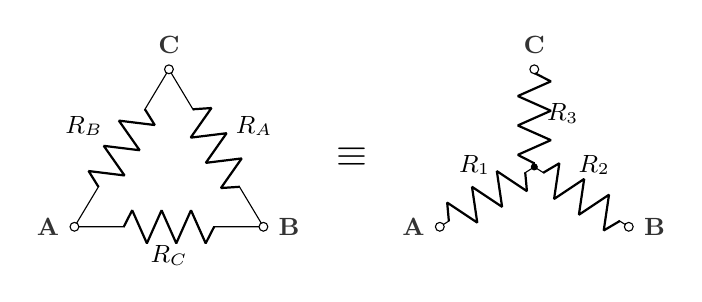
\begin{tikzpicture}[scale=0.8]
  \Dlt{0}
  \node[font=\Large] at (4.4,1.1) {$\equiv$};
  \begin{scope}[shift={(5.8,0)}]
    \Wye{0}
  \end{scope}
\end{tikzpicture}
\end{center}

\textbf{$\boldsymbol{\Delta}$ to Y.} Given $R_A$, $R_B$, $R_C$, find $R_1$, $R_2$, $R_3$. If the
two are equivalent, the resistance between any two terminals, with the third one open, is the
same. Between A and B, the $\Delta$ is $R_C$ in parallel with $R_A + R_B$, and the Y is
$R_1 + R_2$:
\[
  \frac{R_C(R_A + R_B)}{\SD} = R_1 + R_2 \ \ (1), \qquad
  \frac{R_A(R_B + R_C)}{\SD} = R_2 + R_3 \ \ (2),
\]
\[
  \frac{R_B(R_C + R_A)}{\SD} = R_3 + R_1 \ \ (3).
\]
Half of the sum of (1), (2) and (3) gives
\[
  R_1 + R_2 + R_3 = \frac{R_A R_B + R_B R_C + R_C R_A}{\SD} \qquad (4),
\]
and (4)$-$(2), (4)$-$(3), (4)$-$(1) give the result.

\begin{ideabox}[$\Delta$ to Y]
\[
  \Icol{R_1} = \frac{R_B R_C}{\SD}, \qquad
  \Icol{R_2} = \frac{R_C R_A}{\SD}, \qquad
  \Icol{R_3} = \frac{R_A R_B}{\SD}
\]
The Y resistor at a terminal is the product of the two $\Delta$ resistors at that terminal,
divided by the sum of the $\Delta$ resistors.
\end{ideabox}

\textbf{Y to $\boldsymbol{\Delta}$.} Given $R_1$, $R_2$, $R_3$, find $R_A$, $R_B$, $R_C$. From
the result above,
\[
  S = R_1R_2 + R_2R_3 + R_3R_1 = \frac{R_A R_B R_C\,(\SD)}{(\SD)^2} = \frac{R_A R_B R_C}{\SD},
\]
\[
  R_A R_1 = R_B R_2 = R_C R_3 = \frac{R_A R_B R_C}{\SD} = S .
\]

\begin{ideabox}[Y to $\Delta$]
\[
  \textcolor{metured}{R_A} = \frac{S}{R_1}, \qquad
  \textcolor{metured}{R_B} = \frac{S}{R_2}, \qquad
  \textcolor{metured}{R_C} = \frac{S}{R_3}, \qquad
  S = R_1R_2 + R_2R_3 + R_3R_1
\]
A $\Delta$ resistor is the sum of the products of the Y resistors, divided by the Y resistor
opposite to it.
\end{ideabox}

\begin{minipage}[c]{0.56\linewidth}
\textbf{Equal resistors.} A $\Delta$ of three equal resistors $R$ is equivalent to a Y of three
resistors $R \cdot R/(3R) = R/3$. Conversely, a Y of three resistors $R$ is equivalent to a
$\Delta$ of three resistors $3R$.

\smallskip
\textbf{Exercise.} Write both transforms with conductances, $G_\square = 1/R_\square$.
\emph{Answer:} Y to $\Delta$ becomes $G_A = G_2G_3/(G_1 + G_2 + G_3)$, and so on; it has the
form of $\Delta$ to Y with resistances.
\end{minipage}\hfill
\begin{minipage}[c]{0.4\linewidth}
\centering
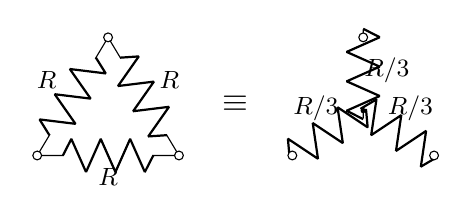
\begin{tikzpicture}[scale=0.6]
  \Dltq
  \node[font=\large] at (4.2,1.1) {$\equiv$};
  \begin{scope}[shift={(5.4,0)}]
    \Wyeq{R/3}
  \end{scope}
\end{tikzpicture}
\end{minipage}

%==============================================================
\section{An example: a bridge}

\begin{examplebox}[Example 13.2 --- a bridge]
\textbf{Question.} Find the resistance $R$ between the two terminals. No two resistors are in
series or in parallel.

\smallskip
\begin{minipage}[c]{0.48\linewidth}
\centering
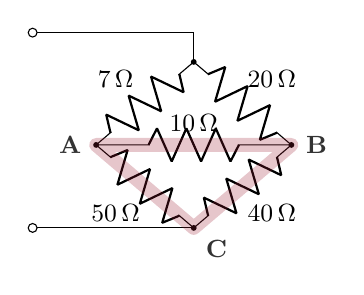
\begin{tikzpicture}[scale=0.62]
  \exBr{1}
\end{tikzpicture}
\end{minipage}\hfill
\begin{minipage}[c]{0.48\linewidth}
\centering
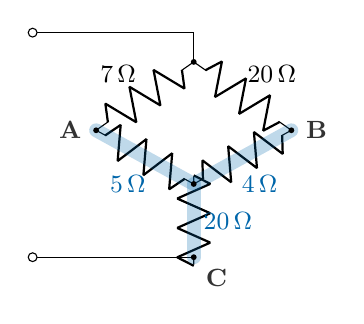
\begin{tikzpicture}[scale=0.62]
  \exBr{2}
\end{tikzpicture}
\end{minipage}

\smallskip
\textbf{Answer.} Transform the $\Delta$ A--B--C into a Y: $R_C = 10\ohm$, $R_B = 50\ohm$,
$R_A = 40\ohm$, and $\SD = 100\ohm$. So
\[
  \Icol{R_1} = \frac{50 \cdot 10}{100} = \Icol{5\ohm}, \qquad
  \Icol{R_2} = \frac{10 \cdot 40}{100} = \Icol{4\ohm}, \qquad
  \Icol{R_3} = \frac{40 \cdot 50}{100} = \Icol{20\ohm} .
\]
In the new circuit, $7 + 5 = 12\ohm$ and $20 + 4 = 24\ohm$ are in parallel, $12 \parallel 24 =
8\ohm$, and this is in series with $20\ohm$:
\[
  R = 8 + 20 = 28\ohm .
\]
\textbf{Check.} With node voltages, a $1\A$ test source between the terminals gives a terminal
voltage of $28\V$. \ \yes
\end{examplebox}

%==============================================================
\section*{Summary}

\begin{center}
\small
\renewcommand{\arraystretch}{1.25}
\begin{tabular}{@{}>{\raggedright}p{5.4cm} >{\raggedright\arraybackslash}p{10.3cm}@{}}
\toprule
\textbf{In the circuit} & \textbf{What to do}\\
\midrule
a one-port of resistors and dependent sources & connect a $1\A$ test source;
  $\Rin = \Vcol{v}/1\A$\\
a $\Delta$ & Y: $R_1 = R_B R_C/(\SD)$, $R_2 = R_C R_A/(\SD)$, $R_3 = R_A R_B/(\SD)$\\
a Y & $\Delta$: $R_A = (R_1R_2 + R_2R_3 + R_3R_1)/R_1$, and so on\\
equal resistors & $\Delta$ with $R$ $\equiv$ Y with $R/3$\\
\bottomrule
\end{tabular}
\end{center}

\end{document}
